\documentclass[11pt]{article}
\ifdefined\pdftrailerid\pdftrailerid{}\fi
\usepackage[T1]{fontenc}
\usepackage{lmodern}
\usepackage[letterpaper,margin=1in]{geometry}
\usepackage{amsmath,amssymb,amsthm,booktabs,array,graphicx,microtype,xcolor,float}
\usepackage{xurl}
\definecolor{ink}{RGB}{26,74,91}
\usepackage[colorlinks=true,allcolors=ink]{hyperref}
\hypersetup{pdftitle={Reduced denominators of binary logarithm and arctangent series},pdfauthor={}}
\newtheorem{theorem}{Theorem}[section]
\newtheorem{proposition}[theorem]{Proposition}
\newtheorem{lemma}[theorem]{Lemma}
\newtheorem{corollary}[theorem]{Corollary}
\DeclareMathOperator{\den}{den}
\DeclareMathOperator{\lcm}{lcm}
\newcommand{\F}{\mathbb F}
\newcommand{\Q}{\mathbb Q}
\newcommand{\Z}{\mathbb Z}
\newcommand{\ind}{\mathbf 1}
\newcommand{\fl}[1]{\left\lfloor #1\right\rfloor}
\newcommand{\cp}{https://github.com/eldernos/MathematicsResearch/blob/a09e011720bc74396a27f4cb3ce2d8a5b3ce5035}
\newcommand{\lean}[3]{\href{\cp/NormalityChecker/#1.lean\#L#2}{#3}}
\newcommand{\noteurl}[2]{\href{\cp/notes/#1.md}{#2}}
\setlength{\emergencystretch}{1.2em}
\newcommand{\inputrows}[1]{\csname @@input\endcsname #1 }
\raggedbottom
\begin{document}
\begin{center}
{\LARGE\bfseries Reduced denominators of binary logarithm\\[2pt] and arctangent series\par}
\vspace{6pt}
{\small Research draft \enspace$\cdot$\enspace 24 November 2026}
\end{center}
\begin{abstract}
Truncating the Taylor series for $\log 2$ at binary exponent $N$ and multiplying by
$2^N$ gives a rational whose reduced denominator has logarithm $N+o(N)$.
A representation using the two arguments $1-2^{-2}$ and $1+2^{-3}$ reduces this
to $N/2+o(N)$. We determine the rate for every finite integer combination of
dyadic logarithms with nonzero sum. Bang's primitive divisor theorem gives the
minimum rate and all cases of equality for representations of a nonzero integer
multiple of $\log 2$. Integral corrections give explicit common denominators for
approximations valid over a linear number of further shifts. Congruences for
their numerators give finite exclusions of binary words. Related results give
rate $2/3$ for specified binary series for $\arctan(1/2)$ and $\pi$, and
denominator estimates in moving windows for Taylor sums of $e$.
The distribution of the binary shifts of these constants remains open here.
\end{abstract}

\section{Two representations of the logarithm}
For an integer $N\ge0$ write $L_N=\lcm(1,\ldots,N)$, with $L_0=1$.
For $y\in\Q$, let $\den(y)$ be its positive reduced denominator, including
$\den(0)=1$. All logarithms are natural. For the standard expansion put
\[
 R_N=\sum_{j=1}^N\frac{2^{N-j}}{j}.
\]
This rational approximates $2^N\log 2$ with error between $0$ and $1/(N+1)$,
by summing the geometric majorant of the omitted terms. A multiplicative
identity between three rational numbers yields a second approximation.

\begin{theorem}\label{th:half}
For every integer $N\ge0$ let
\[
 Y_N=2\sum_{1\le j\le N/2}\frac{2^{N-2j}}j+
       \sum_{1\le j\le N/3}\frac{(-1)^{j+1}2^{N-3j}}j .
\]
Then $\den(Y_N)\mid L_{\lfloor N/2\rfloor}$ and
$0\le 2^N\log 2-Y_N\le4/(N+1)$. Along all integer positions,
\[
 \lim_{N\to\infty}\frac{\log\den(Y_N)}N=\frac12,\qquad
 \lim_{N\to\infty}\frac{\log\den(R_N)}N=1 .
\]
\end{theorem}

The scale $N$ counts binary digits. In the first sum defining $Y_N$ the last
index is $\lfloor N/2\rfloor$, in the second it is $\lfloor N/3\rfloor$.
The prime divisors determining the limits can be read from much shorter
prefixes. In particular, the first omitted prime band for $Y_N$ carries half
the logarithmic weight of $L_N$. The proof appears in Section~\ref{sec:bands}.

Bailey, Borwein and Plouffe \cite{bbp} used modular arithmetic on shifted series
to extract individual digits of $\log 2$ and $\pi$. The denominator studied here
is that of the \emph{sum} of the retained rational terms. For ordinary harmonic numbers,
Sanna \cite{sanna} estimates the indices at which a fixed prime divides the
numerator of $\sum_{j\le n}1/j$. Shiu \cite[Thm.~2]{shiu} characterizes loss
of the full prime power in the harmonic denominator from the short harmonic
sum in the same range $mp^a\le n<(m+1)p^a$. Here the dyadic factor interacts with
reduction at each prime, and primes of order $N$ govern the first-order term.
Rivoal \cite{rivoal} obtains irrationality measures for logarithms with
denominators restricted to grids of the form $L_{\lfloor\nu m\rfloor}^{s} B^m$.
Such estimates quantify proximity of the real number to prescribed grids.
Our denominator formulas concern specific rational points computed from the
series. The logarithmic identities, the arctangent formulas of
Takahashi \cite{takahashi}, and the modular periodicity for $e$ of Sondow and
Schalm \cite{sondow} are antecedents. Priority for the exact rates at a common
binary cutoff and for the uniform estimates on numerator residues remains
undetermined.

\begin{figure}[ht]
\centering
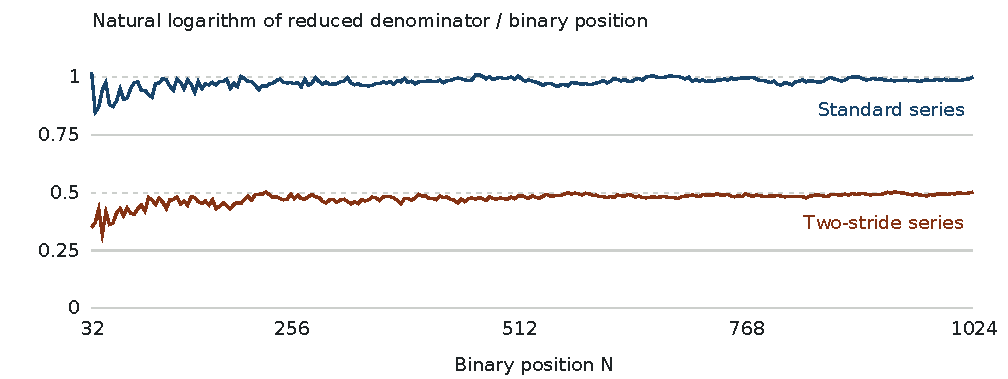
\includegraphics[width=.95\linewidth]{figures/denominators.pdf}
\caption{The reduced denominators in Theorem~\ref{th:half}. Each ordinate uses an
exact rational truncation at $N=32,36,\ldots,1024$, followed by evaluation of its
logarithm. The horizontal dotted lines mark the two proved limits.}
\label{fig:rates}
\end{figure}

\section{Cancellation on prime bands}\label{sec:bands}
Write $\vartheta(t)=\sum_{p\le t}\log p$, the sum being over primes. We use the
prime number theorem in the forms $\vartheta(t)\sim t$ and $\log L_N\sim N$,
and the elementary Chebyshev bound $\log L_k\le7k$.
A rational is integral at $p$ when its reduced denominator is prime to $p$.
Congruences of such rationals use the inverse of the denominator.

\begin{proposition}[Standard logarithm]\label{prop:standard}
Set $P_k=\sum_{j=1}^k2^{-j}/j$ and $q_N=\den(R_N)$. If $p$ is odd prime and
$p^a\le N<p^{a+1}$ for $a\ge1$, then $p^a\mid q_N$ if and only if
$p$ does not divide the reduced numerator of $P_{\lfloor N/p^a\rfloor}$.
For $N\ge8$,
\[
 0\le\log(L_N/q_N)\le116 N^{2/3}.
\]
\end{proposition}
\begin{proof}
Put $L_N=p^a C$ and $k=\lfloor N/p^a\rfloor<p$. In $L_N R_N$ all terms
except those at $j=p^a i$ vanish modulo $p$. For the others,
$2^{p^a i}\equiv2^i\bmod p$, so $L_NR_N\equiv 2^NC P_k\bmod p$.
The factors $2^NC$ and the denominator of $P_k$ are units. This proves the
criterion for the full power.

Let $K=\lceil N^{1/3}\rceil$. For $p\le K^2$, write
$l=\lfloor\log_p K^2\rfloor\ge1$. Since $N\le K^4<p^{2(l+1)}$, the exponent
in $L_N$ is at most $2l+1\le3l$. Thus $L_{K^2}^3$ covers all possible losses
at these primes. For $p>K^2$ with $p\le N$, the only possible loss is one
factor $p$, which must divide the positive numerator of some $P_k$, $1\le k\le K$.
This numerator is at most $2^kL_k$ since $0<P_k<1$. Hence
\[
 \log(L_N/q_N)\le 3\log L_{K^2}+
   \sum_{k=1}^{K} \log(2^kL_k)\le(21+8)K^2 .
\]
Now $K\le2N^{1/3}$, and $q_N\mid L_N$ gives the lower bound.
\end{proof}

\begin{corollary}[Polylogarithms]\label{cor:poly}
For fixed integers $b\ge2$, $s\ge1$, the rational
$R_{b,s}(N)=\sum_{j=1}^N b^{N-j}/j^s$ has
$\log\den(R_{b,s}(N))=s\log L_N+O_{b,s}(N^{2/3})$. For $s=0$
it is an integer.
\end{corollary}
\begin{proof}
The common denominator is $L_N^s$. Keep the small-prime allowance
$L_{K^2}^{3s}$ in the preceding proof and take $N$ large enough that $K^2>b$.
For $p>K^2$, multiplication by $L_N^s$ and reduction modulo $p$ give the
short sum $\sum_{i\le N/p}b^{-i}/i^s$ times the unit $b^N(L_N/p)^s$.
If any of the $s$ powers are lost, its reduced numerator is divisible by $p$.
Each such numerator is positive and at most $b^kL_k^s$ at length $k$, since
the sum is at most one. The product of these bounds for $k\le K$, raised to
the power $s$, has logarithm $O_{b,s}(K^2)$. For $s=0$ each summand is integral.
\end{proof}

For a bounded integer sequence $W(j)$, $j\ge1$, define
\[
 P_v(W)=\sum_{j=1}^v\frac{W(j)}{j2^j},\qquad S_N(W)=2^NP_N(W).
\]
A finite integer combination of $\log(1\pm2^{-k})$ ($k\ge1$) has this
form after grouping equal binary exponents. The contribution of a minus
logarithm with coefficient $b_k$ is $-k b_k\,\ind_{k\mid j}$.
A plus logarithm can be rewritten using
$\log(1+x)=\log(1-x^2)-\log(1-x)$. This identity holds coefficient by
coefficient in its convergent power series, so every cutoff is preserved.

\begin{theorem}[Prime-band formula]\label{th:bands}
Suppose $W(pj)=W(j)$ for every $j\ge1$ and all sufficiently large primes $p$.
With $q_N=\den(S_N(W))$,
\begin{equation}
 \lim_{N\to\infty}\frac{\log q_N}{N}
  =\sum_{\substack{v\ge1\\P_v(W)\ne0}}\left(\frac1v-\frac1{v+1}\right).
 \label{eq:bands}
\end{equation}
This applies to every fixed finite combination above. When its sum is nonzero,
the right side is one minus a finite sum over the vanishing prefixes.
\end{theorem}
\begin{proof}
For an odd prime satisfying the invariance and $p^2>N$, the rational
$pS_N(W)$ is integral at $p$. Only $j=p\ell$ can contribute modulo $p$.
Fermat's congruence $2^{p\ell}\equiv2^\ell$ gives
\begin{equation}
 pS_N(W)\equiv 2^N P_{\lfloor N/p\rfloor}(W)\pmod p.
 \label{eq:prime}
\end{equation}
If $S_N(W)=A/q_N$ in lowest terms, a nonzero residue on the right is
equivalent to $v_p(q_N)=1$, in which case it equals $A/(q_N/p)\bmod p$.
A zero residue gives $p\nmid q_N$.

Fix $V\ge1$. On $N/(v+1)<p\le N/v$, for $1\le v\le V$, the test uses the
single rational $P_v(W)$. For large enough $N$, all these primes satisfy
the hypotheses and avoid every numerator prime factor of the finitely many
nonzero values. The prime number theorem gives contribution
$N(1/v-1/(v+1))+o_V(N)$ for each nonzero value and zero for a zero value.
Since $q_N\mid L_N$, the remaining first powers cost at most
$\vartheta(N/(V+1))$. All higher powers together cost at most $\sqrt N\log N$.
Taking the upper and lower limits and then letting $V\to\infty$ proves
\eqref{eq:bands}. For the finite logarithm combinations, primes coprime to all
strides preserve each divisibility indicator. When the sum is nonzero,
convergence implies that $P_v(W)\ne0$ for all sufficiently large $v$.
\end{proof}

\begin{proof}[Proof of Theorem~\ref{th:half}]
The identity $(1+2^{-3})/(1-2^{-2})^2=2$ gives the two Taylor series defining
$Y_N$. Absolute convergence permits grouping them by binary exponent. Their
weights, starting at $j=1$, repeat $(0,4,3,4,0,1)$, equivalently
\[
 w(j)=4\,\ind_{2\mid j}+3\,\ind_{3\mid j}-6\,\ind_{6\mid j}.
\]
The nonnegative tail is bounded by $4\sum_{i\ge1}2^{-i}/(N+1)$.
In the ungrouped sums every retained denominator divides $L_{\lfloor N/2\rfloor}$.
The only positive index $v$ with $P_v(w)=0$ is $v=1$.
Equation~\eqref{eq:bands} now gives rate $1/2$. The second limit follows from
Proposition~\ref{prop:standard} and $\log L_N\sim N$.
\end{proof}

For example, when $N/3<p\le N/2$, $p>3$ and $p^2>N$,
\eqref{eq:prime} reads $pY_N\equiv 2^{N-1}\pmod p$ since $P_2(w)=1/2$.
At $N=10$ the two prefixes are $R_{10}=44711/63$ and $Y_{10}=10646/15$.

\begin{theorem}[Optimality in the finite dyadic class]\label{th:optimal}
Fix $m\in\Z\setminus\{0\}$. Represent $m\log 2$ as a finite integer linear
combination of $\log(1\pm2^{-k})$ with positive integer strides $k$ fixed
independently of $N$. Truncate at binary exponent $N$ and multiply by $2^N$.
The least possible limiting rate \eqref{eq:bands} is $1/2$. Equality holds
precisely when the grouped weights are $m w(j)$ for every $j$.
\end{theorem}
\begin{proof}
Rewrite the plus logarithms as above, and denote the resulting coefficients
of $\log(1-2^{-k})$ by $b_k$. Exponentiation gives
$\prod_k(2^k-1)^{b_k}2^{-\sum_k k b_k}=2^m$.
If the largest occupied $k$ exceeds six, Bang's theorem \cite{bang} supplies
a prime divisor of $2^k-1$ dividing none of $2^i-1$ for $1\le i<k$.
Its valuation in the identity forces $b_k=0$, a contradiction. Among the
remaining indices the valuations at $31$ and $5$ give $b_5=b_4=0$.
At $7$ and $3$ they give $b_3=-b_6$ and $b_2=-2b_6$, respectively, since
$2^6-1=3^2\cdot7$. The valuation at $2$ gives $m=b_6-b_1$. Thus
$W(j)=-b_1+b_6 w(j)$. If $b_1=0$, then $W=m w$ and the rate is $1/2$.
Otherwise $P_1(W)=-b_1/2\ne0$, contributing $1/2$ by itself.
Since $P_v(W)\to m\log2\ne0$, some later band also contributes.
\end{proof}

The quantifiers allow arbitrarily large finite stride lists and coefficients.
Changing the cutoff, permitting coefficients to depend on $N$, or adding
geometrically decaying rational corrections changes the problem. For example,
$\log2=2\sum_{j\ge0}3^{-(2j+1)}/(2j+1)$ uses powers of $3$ throughout.
Another larger class arises from complex logarithms. Adegoke, Lafont and
Layeni \cite[eqs.~(28)--(29)]{adegoke} give a binary formula for $\log2$
using two complex arguments of modulus $1/\sqrt2$. Their formula and the
base-three series above are outside Theorem~\ref{th:optimal}.

\section{Signed integral corrections}\label{sec:correct}
Write $B(m,j)=\int_0^1t^m(1-t)^j\,dt=m!j!/(m+j+1)!$ for nonnegative integer
arguments. For $a\in\{2,4,-8\}$ set
\begin{align*}
 I_a&=\int_0^1\frac{dt}{a-t}=\log\left|\frac{a}{a-1}\right|,\\
 C_a(m,r)&=\sum_{j=1}^m\frac{a^{m-j}}{j}
       +\sum_{j=0}^{r-1}\frac{(-1)^jB(m,j)}{(a-1)^{j+1}} .
\end{align*}
Here $2I_4-I_{-8}=\log 2$. Let $m_k=\lfloor N/k\rfloor$ and $t_k=N-km_k$.
The signed multipliers, including the incomplete last stride, are
$\lambda_2=2^{1+t_2}$ and $\lambda_3=-(-1)^{m_3}2^{t_3}$.

\begin{theorem}\label{th:correct}
For all integers $N,r,s\ge0$ put
\[
 Z=\lambda_2 C_4(m_2,r)+\lambda_3 C_{-8}(m_3,s),\qquad
 M=\max(m_2+r,m_3+s),\quad K=3^{\max(r,2s)} .
\]
Then $\den(Z)\mid KL_M$, and
\begin{equation}
 |2^N\log 2-Z|\le
 \eta=\frac{2^{1+t_2}B(m_2,r)}{3^r}+
       \frac{2^{t_3}B(m_3,s)}{9^s}.
 \label{eq:error}
\end{equation}
For every $i\ge0$ the same $Z$ satisfies $|2^{N+i}\log 2-2^iZ|\le2^i\eta$.
\end{theorem}
\begin{proof}
Finite geometric division of $a^m/(a-t)$ gives the first sum in $C_a$ upon
integration and leaves $t^m/(a-t)$. Expand the latter denominator about $t=1$
by dividing $1$ by $(a-1)+(1-t)$. Integrating the finite geometric identity gives
\begin{equation}
 a^m I_a-C_a(m,r)=\frac{(-1)^r}{(a-1)^r}
   \int_0^1\frac{t^m(1-t)^r}{a-t}\,dt .
 \label{eq:beta}
\end{equation}
The three allowed values of $a$ satisfy $|a-t|\ge1$. Multiplying
\eqref{eq:beta} by the two $\lambda_k$ gives \eqref{eq:error}, also when
$r$ or $s$ vanishes. The binomial expansion
\[
 B(m,j)=\sum_{\ell=0}^j\frac{(-1)^\ell\binom j\ell}{m+\ell+1}
\]
has denominator dividing $L_{m+j+1}$. In each correction the remaining factor
has denominator dividing $3^r$ or $9^s$. Both divide $K$, and every denominator index
in the expansion is at most $M$. This gives a single common denominator $KL_M$.
\end{proof}

\begin{corollary}[Budgets for linear coverage]\label{cor:budgets}
Let $\alpha,\rho,\sigma>0$, set $r=\lceil\rho N\rceil$,
$s=\lceil\sigma N\rceil$, and define
\[
 F(\beta,u,d)=(\beta+u)\log(\beta+u)-\beta\log\beta-u\log u+u\log d.
\]
If $\min(F(1/2,\rho,3),F(1/3,\sigma,9))\ge\alpha\log2$, then
$2^{\lfloor\alpha N\rfloor}\eta\to0$ and
\[
 \lim_{N\to\infty}\frac{\log(KL_M)}N=
 C=\max(1/2+\rho,1/3+\sigma)+\max(\rho,2\sigma)\log3 .
\]
In particular $\limsup_N N^{-1}\log\den(Z)\le C$. Table~\ref{tab:budgets}
gives strict upper bounds for $C$.
\end{corollary}
\begin{proof}
With $m=\lfloor\beta N\rfloor$, $j=\lceil uN\rceil$, Stirling's formula
in $1/((m+j+1)\binom{m+j}{j})$ gives
$d^{-j} B(m,j)=O_{\beta,u,d}(N^{-1/2}e^{-NF(\beta,u,d)})$.
Rounding changes the exponential by a bounded factor since both proportions
are positive. The factor $N^{-1/2}$ handles equality at the last shift.
The formula for $C$ follows from $\log L_M=M+o(M)$.
For each row in the table clear the denominators of $\beta,u,\alpha$ by $v$
and put $(b,j,h)=v(\beta,u,\alpha)$. The strict comparison amounts to
$(b+j)^{b+j}d^j>2^h b^b j^j$. The two integer comparisons hold in each row.
For the last column bound $\log3=2\sum_{j\ge0}2^{-(2j+1)}/(2j+1)$
using the terms $j<13$ and a tail at most
$2\cdot 2^{-27}/(27(1-1/4))$. These rational comparisons are reproduced
with the table data.
\end{proof}

\begin{table}[ht]
\centering
\caption{Certified common-denominator rates. The horizon is $\lfloor\alpha N\rfloor$
further binary shifts. The reduced denominator can be smaller.}\label{tab:budgets}
\begin{tabular}{rrrr}\toprule
$\alpha$ & $\rho$ & $\sigma$ & upper bound for $C$\\\midrule
\inputrows{figures/budgets.tex}
\bottomrule\end{tabular}
\end{table}

\section{Congruences for prescribed numerators}\label{sec:num}
At a surviving prime the residue of the unreduced numerator can determine the reduced numerator locally. For $Z$ in
Theorem~\ref{th:correct}, let $B_0=KL_M Z\in\Z$. By the binomial expansion
in that proof, $KZ=\sum_{j=1}^M u_j/j$ for explicit $u_j\in\Z$:
multiply each raw prefix coefficient by $K\lambda_k$ and distribute each
correction $K\lambda_k(-1)^i B(m_k,i)/(a-1)^{i+1}$ among
$j=m_k+\ell+1$ using $(-1)^\ell\binom i\ell$, $0\le\ell\le i$.

\begin{proposition}\label{prop:local}
For $p^v\Vert L_M$, with $d_j=v_p(j)$, the cleared numerator satisfies
\[
 B_0\equiv\frac{L_M}{p^v}
   \sum_{\substack{j\le M\\p\mid j}}
       u_j\,p^{v-d_j}(j/p^{d_j})^{-1}\pmod{p^v}.
\]
Modulo $K$, it is the sum of the correction terms alone, each multiplied
by $KL_M$. If $Z=A/q$ is in lowest terms then
$v_p(q)=\max(0,v_p(KL_M)-v_p(B_0))$, with $v_p(0)=+\infty$.
\end{proposition}
\begin{proof}
In $B_0=\sum_j u_j(L_M/j)$ the terms with $p\nmid j$ vanish modulo $p^v$.
Factoring the numerator and denominator powers of $p$ in each remaining term
gives the formula. Every raw prefix term of $KL_M Z$ is divisible by $K$,
since its index divides $L_M$. Finally $q=KL_M/\gcd(KL_M,B_0)$.
For $p\ne3$, a unit value modulo $p^v$ therefore retains the full power in $q$
and determines $A\bmod p^v$ by multiplication by the inverse of $KL_M/q$.
At $3$, the power in $L_M$ and the extra factor $K$ may overlap.
\end{proof}

For the single standard series consider the diagonal correction
$y_n=C_2(n,n)$. Its error is at most
$\eta_n=B(n,n)=1/((2n+1)\binom{2n}{n})$ by \eqref{eq:beta}, and
$\den(y_n)\mid L_{2n}$. The index $n=0$ gives $y_0=0$.
The following estimate counts returns to \emph{each} field element.

\begin{theorem}[Diagonal numerator residues]\label{th:diagonal}
Let $\delta_n=y_{n+1}-2y_n$ and $U_n=3y_n/\delta_n$. Then
\begin{equation}
 \delta_n=\tfrac32(-1)^nB(n,n),\qquad
 (n+1)U_{n+1}=-2(2n+3)(2U_n+3).
 \label{eq:diagonal}
\end{equation}
For a prime $p>3$, $U_n$ is integral at $p$ on $0\le n<p$. For every
$c\in\F_p$ and $0<h<p/2$ there are at most $h$ indices
$0\le n<n+h<p$ with $U_n=U_{n+h}=c\bmod p$. In particular a prescribed
residue occurs $O(T^{2/3})$ times in any $T$ consecutive positions of
$[0,p)$. When $n<p\le2n$ this is a restriction on $p y_n$ multiplied by
the explicit unit $3/(p\delta_n)$.
\end{theorem}
\begin{proof}
Subtract twice \eqref{eq:beta} at $(n,n)$ from the same formula
at $(n+1,n)$. This gives $C_2(n+1,n)-2C_2(n,n)=(-1)^nB(n,n)$.
The additional term is $(-1)^n B(n+1,n)=(-1)^n B(n,n)/2$.
Thus $\delta_{n+1}/\delta_n=-(n+1)/(2(2n+3))$ and \eqref{eq:diagonal} follows.
Induction shows $n!U_n\in\Z$. On the stated band the factorial quotient
$B(n,n)$ has valuation $-1$, since $2n+1<2p$.

Iterate the recurrence from the symbolic index $X$ and the value $c$.
After $j$ steps the fraction is $A_j/D_j$, starting with $A_0=c,D_0=1$, where
\[
 D_{j+1}=(X+j+1)D_j,\qquad
 A_{j+1}=-2(2X+2j+3)(2A_j+3D_j).
\]
Both degrees are at most $j$ at step $j$. A return at gap $h$ requires a
root of $A_h-cD_h$ in $\F_p$. For $c\ne0$ evaluate at $X=-h-1/2$.
The last numerator vanishes, while twice each factor of $D_h$ is a
nonzero odd integer in absolute value at most $2h-1$. For $c=0$ evaluate
at $X=-1$. Then $A_1=-6$, and for $j\ge1$, $D_j=0$ and
$A_{j+1}=-4(2j+1)A_j$ there. All factors are units through step $h$.
The polynomial is nonzero in either case, so has at most $h$ roots.
The permitted starts are distinct in the field. Partition a length-$T$
interval into bins of at most $H+1$ consecutive positions. Each occurrence
after the first in a bin gives a distinct pair at gap at most $H$.
The bound is $\lceil T/(H+1)\rceil+H(H+1)/2$. Taking
$H=\max(1,\lfloor T^{1/3}\rfloor)$ gives the assertion ($2H<p$ for $p>3$).
\end{proof}

This also explains why large diagonal denominators persist in moving
windows. We record a proof, since the quantifier over the starting position
differs from ordinary density one.

\begin{corollary}\label{cor:uniform}
For each $\epsilon>0$, each of the following sets has upper Banach density zero:
indices $n$ with $\log\den(y_n)\le(1-\epsilon)n$, and indices where at least
a fraction $\epsilon$ of the primes in $(n,2n]$ are absent from $\den(y_n)$.
Here upper Banach density zero means that the exceptional proportion in
$[x,x+T)$ tends to zero as $T\to\infty$, uniformly over integers $x\ge0$.
\end{corollary}
\begin{proof}
Put $E_n=\sum_{n<p\le2n,\ p\nmid\den(y_n)}\log p$. For $p>3$ in this band
a missing prime is equivalent to $U_n=0\bmod p$, by \eqref{eq:diagonal}
and $\den(y_n)\mid L_{2n}$. At each $p$ the eligible indices form an interval
in $[0,p)$, hence Theorem~\ref{th:diagonal} bounds their missing count in a
window of length $T$ by $O(T^{2/3})$. The primes $2,3$ contribute only
boundedly. Summing first over $p$ gives
$\sum_{x\le n<x+T}E_n\ll (x+T)T^{2/3}$.
By the prime number theorem $\vartheta(2n)-\vartheta(n)\sim n$ and
$\#\{n<p\le2n\}\sim n/\log n$. Either exception costs $E_n\gg_\epsilon n$
for large $n$. If $x\ge T$ this bounds the exceptional fraction by
$O_\epsilon(T^{-1/3})$. For $x<T$ embed the window in $[0,2T)$, discard the
first $\lceil\tau T\rceil$ indices, and charge at least
$c_\epsilon\tau T$ for each remaining exception. The fraction is at most
$\tau+O_\epsilon(\tau^{-1}T^{-1/3})+O(T^{-1})$. Let $T\to\infty$ then
$\tau\downarrow0$.
\end{proof}

\section{Large primes and binary word exclusions}\label{sec:sieve}
Let $L$ be a common denominator for a rational $z$ satisfying
$|2^n\log2-z|\le\eta$. Suppose that congruences determine
$Lz\equiv r\bmod P$, where $P\mid L$, $0\le r<P$, and write $H=L/P$.
Given these congruences, the possible fractional parts are exactly
$r/L+j/H\bmod1$, $0\le j<H$. A binary word of length $T$ with integer value
$u$ (leading zeroes allowed) occupies the half-open interval
$[u/2^T,(u+1)/2^T)$. Using the closed enlargement gives the necessary test
\begin{equation}
 \left\lceil\frac{L(u2^{-T}-\eta)-r}{P}\right\rceil
 \le
 \left\lfloor\frac{L((u+1)2^{-T}+\eta)-r}{P}\right\rfloor .
 \label{eq:grid}
\end{equation}
Indeed the closed interval must contain an integer lift $r+Pj$ after scaling.
Allowing all $j\in\Z$ handles the cut at zero. Failure proves exclusion for
the real number. Passing only certifies compatibility with the given data.

\begin{proposition}[Two choices of modulus]\label{prop:lift}
For $z=y_n$, $n\ge1$, take $M=2n$, $L=L_M$ and
$P=\prod_{\sqrt M<p\le M}p$. Then $\log H=(2+o(1))\sqrt M$.
For $z=Z$ of Theorem~\ref{th:correct}, use $L=K L_M$ and, for
$3\le y<M$, use $P=K\prod_{p>y,\ p^v\Vert L_M}p^v$ (positive exponents).
Then
\[
 H=\prod_{p\le y}p^{\lfloor\log_p M\rfloor},\qquad
 \log H=(\lfloor1/\gamma\rfloor+o(1))M^\gamma\quad
 \text{if }y=M^\gamma,\quad 0<\gamma<1 .
\]
Each modulus gives the residue of the specified rational using only indices
divisible by the tested prime, together with the correction residue modulo
$K$ in the second case.
\end{proposition}
\begin{proof}
For the diagonal model write $y_n=\sum_{k=1}^{2n} a_k/k$. For $k\le n$,
$a_k=2^{n-k}$. The remaining coefficient $a_{n+\ell+1}$ is the coefficient
of $t^\ell$ in $\sum_{j=0}^{n-1}(-1)^j(1-t)^j$, by the beta integral.
Thus $Ly_n\bmod p$ equals $(L/p)\sum_{i\le2n/p}a_{pi}/i\bmod p$ for
$p>\sqrt{2n}$. The Chinese remainder theorem combines the residues, including
zero values. The unrecovered logarithmic weight is
$\vartheta(\sqrt M)+\sum_{a=2}^{\lfloor\log_2 M\rfloor}\vartheta(M^{1/a})$.
The first two terms are each asymptotic to $\sqrt M$, and the rest total
$O(M^{1/3}\log M)$.

For $Z$, Proposition~\ref{prop:local} gives all the required residues.
The tested prime powers are coprime to $K$, since $y\ge3$. Removing these
factors from $L$ leaves exactly $H$ as displayed, including the ordinary
$3$-part of $L_M$. Now
$\log H=\sum_{a\ge1}\vartheta(\min(y,M^{1/a}))$. The first
$J=\lfloor1/\gamma\rfloor$ terms equal $\vartheta(y)$, including equality
at $1/\gamma\in\Z$. The remainder is $O(M^{1/(J+1)}\log M)=o(y)$.
\end{proof}

For the diagonal model with $T=n$, the interval in \eqref{eq:grid} has length
$H(2^{-n}+2\eta_n)=o(1)$, since $\binom{2n}{n}\ge 4^n/(2n+1)$.
It contains at most one integer for large $n$. For fixed $T$, by contrast,
$H\ge 2^T$ eventually, so every length-$T$ cylinder already contains a
point of each translated grid before enlargement.

\begin{proposition}[Growing words]\label{prop:entropy}
Fix $0<\gamma<\delta<1$, $c>\log 2$, $0<\rho<1/2$.
At binary position $n$ in the two-stride model take $T=\lfloor n^\delta\rfloor$,
$r=s=\lceil cT/\log(n/T)\rceil$ and $y=M^\gamma$. Then
$2^T\eta\to0$, $\log H=o(T)$, and each local sum at $p>y$ involves
$O(M^{1-\gamma})$ terms. Among all $P$ residues, the proportion passing
\eqref{eq:grid} for at least one word with at most
$\lfloor\rho(T-1)\rfloor$ changes is at most
$\exp(-(\log2-h(\rho)+o(1))T)$, where
$h(\rho)=-\rho\log\rho-(1-\rho)\log(1-\rho)$.
\end{proposition}
\begin{proof}
For $m=m_2,m_3\asymp n$, the factorial formula gives
$B(m,r)\le r!/(m+1)^{r+1}\le(r/(m+1))^r/(m+1)$.
Here $\log((m+1)/r)=\log(n/T)+O(\log\log n)$, so
$\log\eta\le-(c+o(1))T$. Also $M=n/2+o(n)$ and
Proposition~\ref{prop:lift} gives the claimed lift count. For any list
of $W$ words, each enlarged interval of length $2^{-T}+2\eta$ contains
at most $L(2^{-T}+2\eta)+1$ points of the unwrapped $1/L$ grid.
Reduction modulo $P$ then gives the proportion bound
\[
 \min\bigl(1,W[H(2^{-T}+2\eta)+1/P]\bigr).
\]
There are $2\sum_{j\le\lfloor\rho(T-1)\rfloor}\binom{T-1}j$ words (sum from
$j=0$). This is at most $2e^{(T-1)h(\rho)}$ by the binomial theorem
with weights $\rho^j(1-\rho)^{T-1-j}$. Finally $\log P\ge\log L_M-\log H=n/2+o(n)$. These bounds give the result.
\end{proof}

The proportion in this proposition averages over candidate residues at a
single start. The logarithm supplies one particular $r$ there. Concluding
positive density of transitions would require an estimate over actual starts
for those particular residues.

\begin{proposition}[Overlapping observations]\label{prop:overlap}
Suppose a circle phase is within $\eta_1$ of some point of $u+\frac1h\Z/\Z$
and within $\eta_2$ of some point of $v+\frac1k\Z/\Z$, where $h,k\ge1$.
Write $d=\lcm(h,k)$, $g=\gcd(h,k)$. If $2d(\eta_1+\eta_2)<1$, there are
exactly $g$ ordered pairs at circle distance at most $\eta_1+\eta_2$.
Their common error intervals are translates of one interval by $j/g$,
$0\le j<g$. An observation made $\ell$ binary shifts earlier enters this
statement with offset $2^\ell u$, size $h/\gcd(h,2^\ell)$ and error
$2^\ell\eta_1$.
\end{proposition}
\begin{proof}
The differences form $u-v+d^{-1}\Z/\Z$, each attained $hk/d=g$ times
by the difference homomorphism. At most one difference lies within
$\eta_1+\eta_2$ of zero and the actual pair supplies one. The common kernel
is simultaneous translation by the subgroup of order $g$. Since
$\eta_1+\eta_2<1/2$, each compatible pair has lifts with unique signed
difference in $[-(\eta_1+\eta_2),\eta_1+\eta_2]$. Intersecting the two
closed real error intervals and projecting to the circle gives the stated
interval. Multiplication by $2^\ell$ on the earlier grid has image of the
specified size and multiplies the error by at most $2^\ell$.
\end{proof}

For Table~\ref{tab:words} the diagonal error is $B(n,n)$. In the two-stride
rows each correction order is the least one making its own term in
\eqref{eq:error} at most $2^{-T}/(2(T+1))$. For each set of at most $a$
transition sites among $T-1$ gaps, start with each of the two possible
initial digits. Applying \eqref{eq:grid} with integer ceilings and floors
gives the last column.

\begin{table}[H]
\centering\small
\caption{Exact exclusions for $\log 2$. The index $n$ counts preceding digits,
$a$ is the maximum number of changes and $y$ is the integer prime cutoff.
The bits column gives $\lfloor\log_2 H\rfloor+1$. The last column counts words
passing the closed test, with every unresolved lift allowed.}\label{tab:words}
\begin{tabular}{lrrrrrrrr}\toprule
Model & $n$ & $T$ & $a$ & $y$ & orders & bits & words & pass\\\midrule
\inputrows{figures/sieves.tex}
\bottomrule\end{tabular}
\end{table}

A joint test uses the models at $512$ and $513$, each with orders chosen by
the same rule at $T=64$. Omit the ordinary primes $\{2,3,5\}$ and
$\{2,3,7\}$ respectively, retaining both correction residues modulo $K$.
Advance the first observation one bit. The resulting grid sizes are
$h=3\,888\,000$ and $k=3\,048\,192$, and the narrowness inequality in
Proposition~\ref{prop:overlap} holds. There are $g=31\,104$ compatible pairs.
To enumerate their joint words, let $b$ be the unique integer satisfying
$|u-v+b/d|\le\eta_1+\eta_2$. Solve
$(k/g)i-(h/g)j=b$ and intersect the two intervals about $u+i/h$ and $v+j/k$.
If their intersection is $[l,t]$, the closed cylinders admitted at this pair
have word integers from $\lceil2^{64}l\rceil-1$ through $\lfloor2^{64}t\rfloor$,
reduced modulo $2^{64}$. Apply the same formula to all $g$ translates.
Exactly $31\,232$ distinct words remain, of which one has $18$ changes
and none has fewer. Thus the $64$ bits following position $513$ in $\log 2$
have at least $18$ changes. This lower bound concerns that single word.

\section{Arctangents and the number \texorpdfstring{$\pi$}{pi}}\label{sec:angles}
Let $\chi(j)=0$ for even $j$ and $\chi(j)=(-1)^{(j-1)/2}$ for odd $j$.
It is the real Dirichlet character modulo four. First consider the usual
Taylor truncations.

\begin{corollary}\label{cor:dyadic}
For fixed $k\ge1$, each of $-\log(1-2^{-k})$, $\log(1+2^{-k})$ and
$\arctan(2^{-k})$ has a Taylor prefix at binary exponent $N$ whose shift
by $2^N$ has reduced-denominator rate $1/k$. More generally the Taylor
series for $\arctan(1/b)$, $b\ge2$ an integer, shifted by $b^m$ and
retained through degree $m$, has reduced-denominator rate one per radix-$b$
position.
\end{corollary}
\begin{proof}
In radix $b$ the three prefixes have the form
$\sum_{j=1}^m b^{m-j} f(j)/j$ with $f(j)=1,(-1)^{j+1},\chi(j)$ respectively.
For odd primes $p\nmid b$ the first two weights satisfy $f(pj)=f(j)$
and the third satisfies $f(pj)=\chi(p)f(j)$ with $\chi(p)=\pm1$.
Fermat's theorem gives \eqref{eq:prime} with $b$ in place of $2$ and the
additional unit $\chi(p)$ in the third case. Every positive-length unshifted
partial sum is positive, as one sees by pairing consecutive nonzero
terms of decreasing absolute value in each alternating sum. The prime-band proof therefore gives
rate one in radix $b$ for all three. Their omitted tail after shifting is
at most $1/((b-1)(m+1))$. Taking $b=2^k$, $m=\lfloor N/k\rfloor$ and
multiplying by $2^{N-km}$ changes the logarithmic denominator by at most
$k\log2$, proving all binary assertions.
\end{proof}

\begin{proposition}[Two digits at one prime]\label{prop:twodigits}
For $-\log(1-2^{-k})$, $k\ge1$, and $\arctan(1/2)$ respectively, put
\[
 (B,u,a,c)=(2^k,2^{-k},1,2^{-k})\quad\hbox{or}\quad
 (4,-1/4,2,1/2),\qquad V_m=c B^m\sum_{j=0}^{m-1}\frac{u^j}{aj+1}.
\]
Fix an odd prime $p$, put $s=(p-1)/a$, and take $s+1\le m\le s+p$.
Then $pV_m=G_m+pZ_m$, where $G_m=c B^mu^s$ is a unit and $Z_m$ is integral
at $p$. In any $T$ consecutive indices of this window a prescribed residue
of $pV_m\bmod p^2$, or of $Z_m\bmod p$, occurs $O(T^{2/3})$ times,
uniformly in $p,k$ and the residue.
\end{proposition}
\begin{proof}
The unique index with $p\mid aj+1$ is $s$, where $as+1=p$. Removing
$G_m/p$ leaves $Z_m$. For $0<h<p$, both $V_{m+h}-B^hV_m$ and
$Z_{m+h}-B^hZ_m$ equal $c B^h(Bu)^m f_h(m)$, where
\[
 f_h(X)=\sum_{i=0}^{h-1}\frac{u^i}{a(X+i)+1}.
\]
All denominators are units at valid pairs of indices. Prescribing an ordered
pair of $Z$ residues determines $f_h(m)$ for each of the at most two signs
$(Bu)^m$. For residues $w,z\bmod p^2$ of $pV$, one first needs
$z-B^h w\equiv0\bmod p$, then uses $(z-B^h w)/p\bmod p$ in the same
argument. For every target $t\in\F_p$, clearing the $h$ denominators in
$f_h(X)-t$ gives a polynomial of degree at most $h$. At $X=-1/a$ it has
value $a^{h-1}(h-1)!\ne0$. The window has length $p$, so the number of starts
at gap $h$ is at most $h$ for the logarithm and $2h$ for the arctangent.
The bin argument of Theorem~\ref{th:diagonal} gives the claimed bound.
If $V_m=A/q$ in lowest terms, the tested residue is $A/(q/p)\bmod p^2$.
\end{proof}

The two expansions in the next theorem use binary powers throughout.
The angle identities and the component series appear in
Takahashi \cite[eqs.~(11)--(19)]{takahashi}.

\begin{theorem}[Gaussian logarithms]\label{th:gauss}
Put $z_t=(1-i)/2^t$ for $t=2,3$, $b_t(v)=-\sum_{j=1}^v\Im(z_t^j)/j$,
and $M_t=\lfloor2N/(2t-1)\rfloor$. For positive integers $a,c$, put
\[
 x=a\arctan(1/3)+c\arctan(1/7),\qquad
 V_N=2^N\bigl(a b_2(M_2)+c b_3(M_3)\bigr).
\]
Then $q_N=\den(V_N)$ divides $L_{M_2}$,
\[
 |2^Nx-V_N|\le\frac{a}{M_2+1}+\frac{c}{M_3+1},\qquad
 \log(L_{M_2}/q_N)=O_{a,c}(N^{2/3}).
\]
In particular $\log q_N/N\to2/3$. The choices $(a,c)=(1,1)$ and $(8,4)$
give $\arctan(1/2)$ and $\pi$, respectively.
\end{theorem}
\begin{proof}
The argument of $1-z_t$ is $\arctan(1/(2^t-1))$. The logarithmic Taylor
series is absolutely convergent. Since $(1-i)^2=-2i$,
$-\Im(z_t^j)=w_j2^{-e_t(j)}$, with $e_t(j)=\lceil(2t-1)j/2\rceil$
and $w_j$ repeating $(1,1,1,0,-1,-1,-1,0)$ from $j=1$.
The cutoff $e_t(j)\le N$ is $j\le M_t$. The omitted exponents are distinct
within each component, so their shifted powers of two sum to at most one.
This gives the error bound and the retained terms give $q_N\mid L_{M_2}$.
Writing $A=\arctan(1/3)$, $C=\arctan(1/7)$ gives
$\tan(A+C)=1/2$, $\tan(2A+C)=1$. The sums are in $(0,\pi/2)$ since
$C<A<\pi/6$, proving the two specializations.

For odd primes $p$ with $p^2>M_2$, let $v_t=\lfloor M_t/p\rfloor$.
In $\F_p[i]$ the Frobenius sends $i$ to $\chi(p)i$ and fixes rational
scalars integral at $p$. This identity also holds when the ring splits.
Taking the coefficient of $i$ and retaining the terms at $j=p\ell$ yields
\[
 pV_N\equiv 2^N\chi(p)\bigl(a b_2(v_2)+c b_3(v_3)\bigr)\pmod p .
\]
Each $b_t(v)>0$ for $v\ge1$. Its first term is $1/B$ with $B=2^t$, and
the absolute sum of all subsequent terms is at most
$|z_t|^2/(2(1-|z_t|))=1/(B(B-\sqrt2))<1/B$.
Thus for $p\le M_2$ the combined short sum is positive.

Put $J=\lceil N^{1/3}\rceil$. The first powers at $p\le J^2$ cost $O(J^2)$,
and all higher powers in $L_{M_2}$ cost $O(\sqrt N\log N)=O(J^2)$.
For $J^2<p\le M_2$, each lost prime divides the numerator of the positive
short sum displayed above. Its indices are at most $J$. As $p$ increases,
both indices decrease weakly, so there are at most $2J+1$ different pairs.
Their rational sums have absolute value $O_{a,c}(1)$ and common denominator
$8^J L_J$, whose logarithm is $O(J)$. The sum of the logarithms of all
lost primes is bounded by the logarithm of the product of the corresponding
distinct-pair numerators, hence is $O_{a,c}(J^2)$. The prime number theorem
for $L_{M_2}$ finishes the proof.
\end{proof}

\begin{proposition}[Hexadecimal series for $\pi$]\label{prop:bbp}
Let $c_j=4/(8j+1)-2/(8j+4)-1/(8j+5)-1/(8j+6)$ for $j\ge0$, and put
$V_n=\sum_{j=0}^n16^{n-j}c_j$. Every prime $4n+3<p\le8n+1$ with
$p\equiv1,5\bmod8$ divides $\den(V_n)$. Put $\Delta c_j=c_{j+1}-c_j$ and
$Z_n=V_n+\sum_{j=0}^{n-1}\Delta^j c_{n+1}/15^{j+1}$. For all $i,n\ge0$,
\[
 |16^{n+i}\pi-16^i Z_n|\le\frac{4\cdot16^i}{15\cdot60^n}.
\]
\end{proposition}
\begin{proof}
One summand of $V_n$ has denominator $p$ before combining terms. Its
coefficient is $4$ or $-1$ times a power of $16$, a unit at $p$.
There is exactly one such summand since the offsets are distinct modulo eight
and every denominator is $<2p$.
For the error put $u=t^8$, $w=4-2t^3-t^4-t^5$, so
$c_j=\int_0^1u^jw\,dt$ and $\Delta^j c_{n+1}=\int_0^1u^{n+1}(u-1)^jw\,dt$.
The BBP identity $\pi=\sum_{j\ge0}16^{-j}c_j$ \cite{bbp}
gives $16^n\pi-V_n=\int_0^1u^{n+1}w/(16-u)\,dt$.
Expanding about $u=1$ as in \eqref{eq:beta} leaves the error integral
$15^{-n}\int_0^1u^{n+1}(u-1)^nw/(16-u)\,dt$. The inequalities
$u(1-u)\le1/4$, $|w|\le4$ and $16-u\ge15$ give the bound.
\end{proof}

\section{Factorial truncations of \texorpdfstring{$e$}{e}}\label{sec:e}
Set $A_0=1$, $A_{n+1}=(n+1)A_n+1$, and $Q_n=n!/\gcd(A_n,n!)$.
Then $A_n/n!=\sum_{j=0}^n1/j!$, and $Q_n$ is its reduced denominator.
Here the approximated quantity is $e$ itself. The factorial is a different
denominator scale from that of the binary shifts.

\begin{theorem}\label{th:factorial}
For integers $q\ge1$, $n\ge0$, one has $A_{n+q}\equiv A_n\bmod q$.
For every prime $p$ and integer $h\ge1$, at most $h-1$ starts $0\le n<p$
satisfy $A_n=A_{n+h}=0\bmod p$. For each $\epsilon>0$ the set
$\{n:\log Q_n<(1-\epsilon)\log(n!)\}$ has upper Banach density zero.
\end{theorem}
\begin{proof}
The recurrence resets $A_q$ to $1\bmod q$ and has periodic multipliers,
giving the first identity by induction. Sondow and Schalm
\cite[Prop.~A.5]{sondow} prove also that the least period is $q$.
In particular cancellation modulo $p^v$ is determined by
$A_{n\bmod p^v}\bmod p^v$. Starting from $A_n=0\bmod p$ gives
$A_{n+h}=F_h(n)\bmod p$, where $F_1=1$ and
$F_{h+1}=(X+h+1)F_h+1$. This polynomial has degree at most $h-1$
at step $h$ and $F_h(-h)=1$. The field root bound proves the pair count
even across the end of a period.

Write $D_n=\gcd(A_n,n!)$. In an interval of $T\le p$ consecutive indices
the starts are distinct modulo $p$. Binning as in Theorem~\ref{th:diagonal}
gives at most $\lceil T/(H+1)\rceil+H(H-1)/2\ll T^{2/3}$ zeros, with
$H=\max(1,\lfloor T^{1/3}\rfloor)$. For $T\ge p$, splitting into periods
and a possible partial period gives $O(Tp^{-1/3})$ zeros. In $[x,x+T)$ put
$X=x+T$ and charge at most $X\log p/(p-1)$ at each zero, by Legendre's
formula for $v_p(n!)$. Summing at $p\le T$ and $T<p\le X$ gives
\[
 \sum_{x\le n<x+T}\log D_n\ll
 X\bigl(T+T^{2/3}\log(2X)\bigr).
\]
Indeed $\sum_p(\log p)/((p-1)p^{1/3})$ converges, and
$\sum_{p\le X}(\log p)/(p-1)\ll\log(2X)$ by partial summation of
$\vartheta(X)\ll X$. For $x\ge T$, every exceptional index costs at least
$\epsilon\log(x!)$, giving fraction $O_\epsilon(1/\log(2x)+T^{-1/3})$
for large $T$. For $x<T$, apply the bound on $[0,2T)$, where the sum
is $O(T^2)$, then discard $n<\tau T$. Each remaining exception costs
$\gg_\epsilon\tau T\log(\tau T)$ for fixed $\tau>0$ and large $T$.
Letting $T\to\infty$ and then $\tau\downarrow0$ finishes the proof.
\end{proof}
Sondow and Schalm already use gap polynomials for nearby Taylor numerators
\cite[\S3]{sondow}. Berndt, Kim and Zaharescu \cite{bkz} proved that the
only Taylor sums which are continued-fraction convergents to $e$ are $2$ and
$8/3$. The moving-window conclusion of Theorem~\ref{th:factorial} also follows
from their earlier hypergeometric approximation theorem, with a stronger
exception count \cite[Thm.~1.6 and the end of \S4]{bkzgeneral}.
Indeed write $t_n=A_n/n!$ and let $H(t_n)$ be the maximum of its reduced
numerator and denominator. Then $H(t_n)\le3Q_n$ and
$0<e-t_n\le2/(n+1)!$ for $n\ge1$. If $0<\epsilon<1$ and
$Q_n<(n!)^{1-\epsilon}$, choose $0<\delta<1$ with
$(1-\epsilon)(1+\delta)<1$. Then $|e-t_n|<H(t_n)^{-1-\delta}$ for large $n$.
Their theorem for $\mathstrut_0F_0(1)=e$ bounds the number of these indices up to
$X$ by $O_\delta(\log(2X))$. Its proof bounds their number on each sufficiently
late $[x,(1+\delta^2/8)x]$ by $O_\delta(1)$. A bounded number of such
intervals covers $[x,2x]$. This gives upper Banach density zero directly.
The prime-by-prime proof above exhibits which numerator recurrences force
the weaker density conclusion.

\section{Discrepancy and finite observations}\label{sec:disc}
For integer $b\ge2$ write $x_n=\{b^nx\}$. Define the extreme discrepancy by
\[
 D_N^{(b)}(x)=\sup_{0\le u<v\le1}
 \left|\frac1N\#\{0\le n<N:u\le x_n<v\}-(v-u)\right|,
 \qquad D_\infty^{(b)}(x)=\limsup_{N\to\infty}D_N^{(b)}(x).
\]
In base two a change between the next two digits occurs precisely at
$x_n\in[1/4,3/4)$, with the terminating convention for dyadic rationals.
The \lean{BinaryDiscrepancy}{229}{binary transition criterion} states that
$D_\infty^{(2)}(x)<1$ is equivalent to a positive lower density of changes.
In particular a bound such as \eqref{eq:grid} excluding words with at most
$\rho(T-1)$ changes on disjoint windows of lengths $T\ge2$ would suffice if
such windows fully contained in each sufficiently long prefix occupied a
fixed positive fraction of it. Their internal gaps number at least half
their total length. No such coverage is proved for the actual residues.
For $\log 2$ a \lean{LogTwoTransitions}{220}{finite-prefix estimate} gives
$D_N^{(2)}\le\max(7/8,1-(\lfloor\log_{34}N\rfloor-K)_+/N)$ for some $K$ and
all $N\ge2$, where $a_+=\max(0,a)$.

\begin{proposition}\label{prop:pi-gap}
For every fixed integer $b\ge2$, in particular in bases $10$ and $16$,
there is $c_b>0$ such that $D_N^{(b)}(\pi)\le1-c_b\log N/N$ for all large $N$.
\end{proposition}
\begin{proof}
Write $\|t\|$ for circle distance to zero, $a=1/(2(b+1))$, and let $G_N$
count the $n<N$ with $\|(b-1)b^n\pi\|\ge a$.
Put $y=(b-1)\pi$. The published bound $\mu(\pi)<8$ of
Zeilberger and Zudilin \cite{zz} implies $|y-k/b^m|\ge C_b b^{-8m}$ for all
large $m$ and integers $k$, by applying the bound to $k/((b-1)b^m)$.
If $L$ consecutive indices starting at $m$ miss $G_N$, the nearest integers
$k_j$ to $b^{m+j}y$ satisfy $k_{j+1}=bk_j$, since $(b+1)a<1$.
Hence $|y-k_0/b^m|\le a b^{-(m+L-1)}$, giving $m+L\le8m+O_b(1)$.
Every sufficiently late $[m,9m)$ therefore contains a counted index, and
disjoint such windows give $G_N\gg_b\log N$.

Fix $0<d<a/b$. If a circle arc of length at most $d$ contains both $x_n$
and $x_{n+1}$, then $\|(b-1)x_n\|\le d$. Every $v$ in this arc satisfies
$\|(b-1)v\|\le bd<a$. Its visit count is at most $N-G_N$. An arc containing
no consecutive pair has at most $\lceil N/2\rceil$ visits. Apply these bounds
to short intervals and their complements for positive and negative deviations.
If an interval and its complement both have length at least $d$, either
deviation is at most $1-d$. Thus the discrepancy is bounded by the maximum
of $1-G_N/N$, $1-d$ and $\lceil N/2\rceil/N$ for large $N$, as required.
\end{proof}
The gaps in these finite-prefix bounds tend to zero. None of the results here
establishes $D_\infty^{(2)}<1$ for $\log 2$, $\pi$, $e$, or the rational
arctangents considered above. In particular the proposed bound $0.9999$ for
$\log 2$ remains open.

\section{Formal verification and reproducibility}
The formal sources are pinned to
\href{https://github.com/eldernos/MathematicsResearch/tree/a09e011720bc74396a27f4cb3ce2d8a5b3ce5035}{Checkpoint 11 of \emph{Normality and Discrepancy of Arithmetic Expansions}}
(\texttt{a09e011720bc74396a27f4cb3ce2d8a5b3ce5035}).
Table~\ref{tab:lean} identifies the precise scope of the correspondence.
The Lean band formula assumes that the zero-prefix set is finite. This follows
from convergence for the nonzero logarithm identities in
Theorem~\ref{th:optimal}. The series proof of Theorem~\ref{th:bands} also
covers infinite zero sets. The primitive-divisor hypothesis in Lean is
discharged on paper by Bang's theorem. No new Lean declarations accompany
this manuscript.

\begin{table}[ht]
\small\centering
\caption{Theorem correspondence at Checkpoint 11. Linked entries open the
declaration or the mathematical source for a paper deduction.}\label{tab:lean}
\begin{tabular}{@{}p{.26\linewidth}p{.69\linewidth}@{}}
\toprule
Result & Source and scope\\\midrule
Thm.~\ref{th:half}, Prop.~\ref{prop:standard} (CC-01, 03)
 & \lean{StridedLogarithm}{13}{Series identity},
 \lean{StridedLogarithm}{119}{tail}, \lean{StridedLogarithm}{48}{divisibility},
 \lean{StrideDenominatorRate}{199}{half-rate limit},
 \lean{PrimeCancellation}{164}{prime-power criterion},
 \lean{DenominatorGrowth}{133}{standard loss} and \lean{DenominatorGrowth}{162}{rate}.\\[2pt]
Cor.~\ref{cor:poly}, Thms.~\ref{th:bands}--\ref{th:optimal} (CC-02)
 & \lean{PolylogGrowth}{110}{Polylogarithm loss},
 \lean{LogarithmBands}{89}{band limit for a finite zero set},
 \lean{DyadicRelations}{14}{valuation classification} and
 \lean{DyadicRelations}{94}{optimality with primitive divisors}.\\[2pt]
Thm.~\ref{th:correct}, Cor.~\ref{cor:budgets} (CC-13)
 & \lean{CorrectedStrides}{41}{Signed integral}, \lean{CorrectedStrides}{113}{common denominator},
 \lean{CorrectedStrides}{139}{finite error}. The limiting budgets use Stirling's formula on paper.\\[2pt]
Prop.~\ref{prop:local}, Thm.~\ref{th:diagonal}, Cor.~\ref{cor:uniform} (CC-11, 13)
 & \noteurl{corrected-strides}{Prime-power residues} on paper.
 \lean{DiagonalStep}{12}{diagonal step}, \lean{DiagonalNumerator}{17}{normalization},
 \lean{DiagonalNumerator}{135}{paired residues}, \lean{WindowShadow}{67}{moving-window denominator}
 and \lean{WindowShadow}{72}{prime survival}.\\[2pt]
Props.~\ref{prop:lift}--\ref{prop:overlap}
 & \lean{LogShadowIntegral}{53}{Diagonal error} and
 \lean{ResidueWindows}{11}{rigidity of compatible differences}. Grid counts and
 \noteurl{sublinear-residue-windows}{entropy bounds} are paper deductions.
 The word exclusions are exact finite computations.\\[2pt]
Cor.~\ref{cor:dyadic}, Prop.~\ref{prop:twodigits}, Thm.~\ref{th:gauss} (CC-06, 12)
 & \lean{DyadicLogRates}{40}{Positive dyadic logarithm} at all binary positions.
 The signed and character cases, \noteurl{dyadic-prefix-residues}{two-digit bound}
 and \noteurl{gaussian-arctangent-denominators}{Gaussian rate} have paper proofs.\\[2pt]
Prop.~\ref{prop:bbp}, Thm.~\ref{th:factorial} (CC-08, 09)
 & \lean{BBPShadow}{25}{BBP integral}, \lean{BBPDenominator}{44}{prime band},
 \lean{BBPShadow}{112}{shifted error}, \lean{FactorialNumerators}{23}{Taylor periodicity}
 and \lean{FactorialNumerators}{55}{paired zeros}. The factorial window estimate is deduced on paper.\\[2pt]
Section~\ref{sec:disc} (CC-04, 05)
 & \lean{BinaryDiscrepancy}{229}{Transition criterion},
 \lean{LogTwoTransitions}{220}{finite logarithm gap}. Proposition~\ref{prop:pi-gap}
 is a paper deduction from an external irrationality measure.\\
\bottomrule
\end{tabular}
\end{table}

The source directory \path{papers/05-classical-denominators/} contains the
LaTeX manuscript, bibliography, full declaration list and reviewer guide.
Running \texttt{python3 -B figures/generate.py} there regenerates the figure,
exact denominator data, budget comparisons and all word counts. It uses
the checkpoint's \href{\cp/scripts/strided_logarithm.py}{diagonal sieve}
and \href{\cp/scripts/corrected_strides.py}{two-stride sieve}. All boundary
tests use integer or rational arithmetic. The ordinate of
Figure~\ref{fig:rates} alone uses floating-point logarithms.

\paragraph{Authorship disclosure.}
OpenAI Codex prepared the exposition, proofs in this draft, literature
comparison and computational supplement from the cited checkpoint.
The project owner retains responsibility for mathematical review,
attribution and any submission decision.

\clearpage
\bibliographystyle{plain}
\bibliography{references}
\end{document}
